\chapter{Ordinary Differential Equations}
% this section comes from MIT OCW ODE 18.035c Fall 2011 ed.
We will start by talking about \emph{first-order ordinary differential equations}\footnote{The following text comes from MIT OpenCourseWare notes on ODE 18.035c, Fall 2011 Edition},
that is, ordinary differential equations involving the first derivative.
They appear of the form:
\begin{equation}
  y'=f(x,y).
  \label{eq:fode}
\end{equation}

Let's take a look at the exponential function, which is absolutely invaluable in the study of differential equations.
It looks like
\[ x(t)=e^{at}. \]
\begin{figure}[H]
  \begin{center}
    \includegraphics[width=2in]{continuous/ode/ept.eps}
  \end{center}
  \caption{A plot of $x(t)=e^t$.}
  \label{fig:plotept}
\end{figure}
This function has the following properties:
\begin{enumerate}
  \item $e^0 =1$.
  \item $e^{at+c} = e^c e^{at}$.
  \item $e^{at}$ is never zero.
  \item If $a>0$ then $\lim_{t\to 0} e^{at} = \infty$ and $\lim_{t\to -\infty} e^{at}=0$.
  \item If $a>0$ then $\lim_{t\to 0} e^at$ grows much faster than any polynomial.
    \begin{ex}
      $\lim_{t\to\infty} \frac{e^t}{t^3}=\infty$.
    \end{ex}
    \begin{ex}
      $\lim_{t\to\infty}te^{-t}=0.$
    \end{ex}
\end{enumerate}

In a function such as
\[ f(x)=3x^2+2x+1 \]
$x$ is the \textbf{independent variable}\index{independent variable}.
We can freely set it to any $x \in D$ and the function can then be computed.
When we give a name to the value of the function, as in
\[ y=3x^2 +2x +1 \]
or
\[y=f(x) \]
we say that $y$ is the \textbf{dependent variable}\index{dependent variable}.

We can have systems of equations with more than one dependent variable, as in
\[ x =t^2 -1 \]
or
\[ y=3e^t. \]
Here, the dependent variables $x$ and $y$ depend on the variable $t$.
We can have functions with multiple independent variables as well, such as
\[ x=st^2 -t -s. \]
Here, the independent variables are $s$ and $t$ and the dependent variable is $x$.

Or we can have more than one of each:
\[ x =st^2 -t -s \]
\[ y=3e^{t+s} \]
As an abuse of notation, we can use the dependent variable to denote the function, as in
\[ x=x(t)=t^2 -1.\]
Most of what we do will involve \textbf{ordinary differential equations}\index{ordinary differential equations} (ODEs).
These have only one dependent an one independent variable.

\textbf{Parameters}\index{parameters} are similar to variables.
They can take on different values within a set containing objects which are usually similar.
For example, in integrals we have equations like
\begin{equation}
  \int t^2 \ud t = \frac{t^3}{3}+c
  \label{eq:param1}
\end{equation}
so $c$ is a parameter. Each value of $c$ specifies an entire, similar antiderivative.

Sets are written ${t^3 /3 +c : \text{any number $c$}}$.
This means a set of functions $x=x(t)$ parameterized by $c$.
Sets can depend on more than one parameter, as in
\begin{equation}
  x(t)=c_1 e^{-t}+c_2 e^{-7t}
  \label{eq:param2}
\end{equation}
where $c_1$ and $c_2$ are arbitrary constants.

Equation \eqref{eq:param1} represents a $1$-parameter family of functions.
\eqref{eq:param2} represents a $2$-parameter family of functions.

We will write $\ud y / \ud x$, $y'$, or $D_y$ to mean \emph{the derivative of $y$ with respect to $x$.}
  Only the first way of writing this actually specifies the independent variable, which is $x$.
For second derivatives, we would write
\[ \frac{\ud ^2 y}{\ud x^2}= y''=D^2 y. \]

A differential equation expresses a relation between a function and its derivatives.
For example,
\[ \sqrt{x x^{5}}+\cos{(t)}e^{tx} + (x'' x' x )^6 = \sin{(5t)}. \]

The \textbf{order}\index{order} of a differential equation refers to the order of the highest derivative contained therein.

\textbf{Solving} an ODE means finding a function that satisfies the equation.
For many, this is hard or impossible.
It is easy, however, to check a proper solution.
\begin{ex}
  Verify $y(t)=e^{3t}$ is a solution for
  \[ y'=3y \]
  \begin{sol}
    \begin{align*}
      y&=3e^{3t} \\
      \ddx e^{3t} &=3e^{3t} \\
      3e^{3t} &= 3e^{3t}
    \end{align*}
  \end{sol}
\end{ex}
\begin{ex}
  Show that $y(t)=t^3$ is not a solution for \[y'=\frac{y}{t}.\]
  \begin{sol}
    \begin{align*}
      y'(t)&=3t^2 \\
      3t^2 &\neq \frac{t^3}{t}
    \end{align*}
  \end{sol}
\end{ex}
\subsection{Parameterizing}
\begin{ex}
  Find all solutions for
  \[ x''=2t.\]
  \begin{sol}
    \begin{align*}
      \int 2t \ud t &= 2 \int t \ud t \\
      &= t^2 + c_1 \\
      \int (t+c_1) \ud t &= \frac{t^3}{3}+c_1 t +c_2
    \end{align*}
  \end{sol}
\end{ex}
\subsection{Initial Value Problems}
\begin{ex}
  Solve $x''=2t$ with the initial values $x(1)=1$, $x'(1)=2$.
  \begin{align*}
    x'&= t^2 +c_1 \\
    x'(t) &= t^2 + c_1 \\
    x'(1) &=2 \\
    2&= 1+c_1 \\
    c_1 &=1
  \end{align*}
  \begin{align*}
    1&=\frac{1}{3}+1+c_2 \\
    \frac{-1}{3} &= c_2
  \end{align*}
  \[ x(t) = \frac{t^3}{3}+t-\frac{1}{3} \]
\end{ex}

% in-class section
A common differential equation we will encounter is a \emph{freefall problem}.
Here's an example:

\begin{figure}[H]
  \begin{center}
    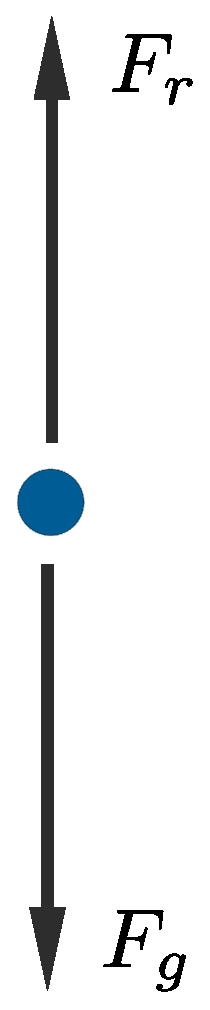
\includegraphics[width=1cm]{continuous/ode/freefall.eps}
  \end{center}
  \caption{A free-body diagram of an object in freefall.}
  \label{fig:freefall}
\end{figure}

Basic physics tells us that $\sum \vec F = m\vec a$,
where $m$ is the object's mass and $\vec{a}$ is the object's acceleration.
For our purposes, we will define $\vec F_g$ to be in the \emph{direction of increasing} $x$.
Based on these assumptions, we can state that
\[
  ma=\vec{F_g}+\vec{F_r}
  \]
Now, acceleration is the same as \emph{change in velocity,} so this is equivalent to
\[
  m\frac{\ud v}{\ud t}=mg - \gamma v
  \]
where $v$ is the object's velocity, $t$ is the time, $g$ is the acceleration of gravity near the surface of Earth, and $\gamma$ is the coefficient of friction for the air.

This is a \textbf{first-order linear ordinary differential equation}.
